\section{Lei de Ohm}


A \textbf{primeira lei de Ohm} é a relação entre as três grandezas elétricas básicas: \textbf{tensão}, \textbf{resistência} e \textbf{corrente}.
%sendo esta a grandeza dependente, ou seja, a que depende das outras duas grandezas, que são independentes.

Considerando o circuito a seguir:

\begin{minipage}{\linewidth}
  \centering
  \begin{minipage}{0.45\linewidth}
    \begin{figure}[H]
      \centering
      \caption{Circuito elétrico simples}
      \label{fig:CircuitoSimples}
      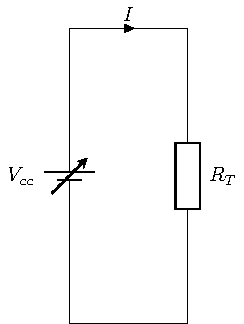
\includegraphics[scale=1.0]{fig-circuitoSimples}

      {\small Fonte: Próprio autor.}
    \end{figure}
  \end{minipage}
  \hspace{0.05\linewidth}
  \begin{minipage}{0.45\linewidth}
    \begin{itemize}
      \item $V_{CC}$: Fonte de tensão ajustável, em Volts[V];
      \item $I$: Intensidade de corrente elétrica, em Amperes [A];
      \item $R_T$: Resistência elétrica em Ohms [$\Omega$].
    \end{itemize}
  \end{minipage}
\end{minipage}

\textbf{Georg Simon Ohm} percebeu que a relação entre tensão e corrente em um circuito resistivo é constante, ou seja, para um dado circuito, com uma resistência fixa, ao variar a tensão aplicada aos seus terminais
a intensidade da corrente que percorre o circuito varia de forma proporcional.

Ao tomar nota de alguns pontos de medição, pode-se desenhar um gráfico como na Figura \ref{fig:leiOhmGrafico}, e perceber que os pontos anotados formam uma reta. Isso ocorre pela proporcionalidade entre a variável manipulada, aquela que é ajustada por quem conduz a experiência, e a variável controlada, que é aquela que depende de outro parâmetro do sistema, e que não é manipulada diretamente.


\begin{figure}[H]
  \centering
  \caption{Grafico $V_{CC}$ x $I$}
  \label{fig:leiOhmGrafico}
  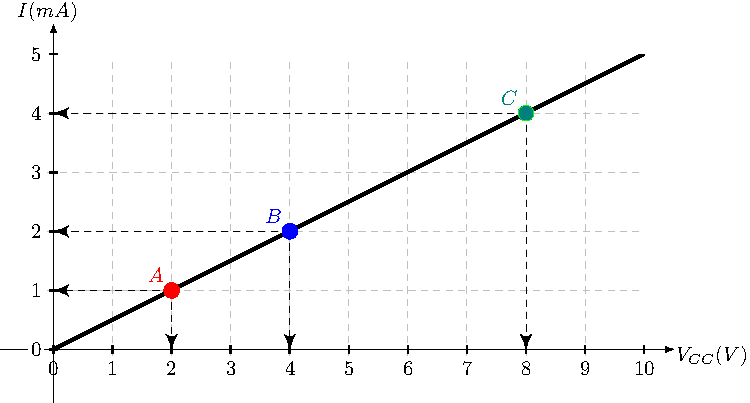
\includegraphics[scale=1.0]{fig-leiOhmGrafico}

  {\small Fonte: Próprio autor.}
\end{figure}

Estão destacados no gráfico três pontos, $A$, $B$ e $C$, e pode-se perceber que o ponto $B$ está localizado em uma tensão que é o dobro da tensão do ponto $A$, por consequência, a intensidade da corrente produzida também é o dobro. O mesmo ocorre no ponto $C$ em relação ao ponto $B$.

A representação matemática para uma reta, é uma equação do primeiro grau, assim a equação que representa a reta do gráfico da Figura \ref{fig:leiOhmGrafico} pode ser obtida da seguinte forma:

Escolha dois pontos quaisquer da reta, $A$ e $B$, $A$ e $C$, $B$ e $C$, ou ainda algum deles com a origem $(0,0)$.

Pontos escolhidos: $B$ e $(0,0)$.

Ao projetar o ponto $B$ no eixo da tensão, temos um triângulo retângulo formado pelos pontos: $B$, $(4,0)$ e $(0,0)$.

Utilizando a relação $\frac{\Delta I}{\Delta V}$, temos o coeficiente algular da reta $G$.

\begin{eqnarray}
  \frac{\Delta I}{\Delta V} & = & G \nonumber \\
  \Delta I & = & G .\Delta V \nonumber \\
  I - I_0 & = & G . (V - V_0)
\end{eqnarray}
Como a origem foi escolhida como um dos pontos do triângulo, o $\Delta I$ será o próprio valor no ponto $B$, ou seja, $I_0$ e $V_0$ valem $0$.

\begin{eqnarray}
  \label{eqn:leiOhmG}
  I & = & G . V
\end{eqnarray}
Analogamente à equação da reta $f(x) = ax + b$ temos que:

\begin{itemize}
  \item $I$ é o resultado da função, é a variável dependente pois varia em função da variável independete;
  \item $V$ é a variável independente, é manipulada por quem conduz o experimento, ajustando o valor da fonte para um valor desejado;
  \item $G$ é coeficiente angular, valor que exprime o quanto a reta está inclinada.
\end{itemize}

O coeficiente angular $G$ mostra que, para um ânglo de inclinação pequeno, uma variação de tensão alta produz uma variação de corrente é pequena, ou seja, a condução é ruim. Com um ângulo de inclinação grande, uma variação de tensão pequena produz uma grande variação de corrente, ou seja, uma ótima condução.

O coeficiente angular $G$ é denominado como \textbf{condutância}, e sua unidade é o \textbf{Siemens[S]}.

A condutância é o inverso da resistência, ou seja, dois aspectos de um mesmo fenômeno.

\begin{eqnarray}
  \label{eqn:GinvR}
  G & = & \frac{1}{R}
\end{eqnarray}

Substituindo (\ref{eqn:GinvR}) em (\ref{eqn:leiOhmG}), temos a \textbf{Primeira Lei de OHM}.

\begin{eqnarray}
  \label{eqn:leiOhmR}
  I & = & \frac{1}{R} . V
\end{eqnarray}
